\section{Versuchsaufbau} % (fold)
\label{sec:durchf_uhrung}
	Zu diesem Versuch liegen Ultraschallsonden bereit, die jeweils verschiedene Frequenzen liefern.
	Sie betragen $\nu_1 = \SI{1}{\mega \hertz}$, $\nu_2 = \SI{2}{\mega \hertz}$ und $\nu_4 = \SI{4}{\mega \hertz}$.
	Die Sonden k"onnen je als Empfangs- und Sendeteil genutzt werden und sind "uber ein Steuerger"at mit einem Computer verbunden.

	\begin{wrapfigure}{r}{6cm}
		\centering
		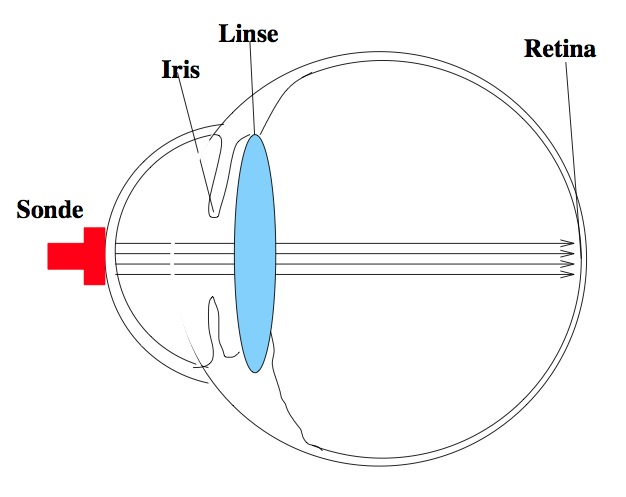
\includegraphics[width = 6cm]{img/auge.jpeg}
		\caption{Aufbau des Augenmodells \label{fig:auge}}
	\end{wrapfigure}

	Dieser zeigt ein Amplituden-Laufzeit-Diagramm der aktiven Sonde an (A-Scan) oder kann bei Bewegung der Sonde ein Bild aufnehmen (B-Scan).
	Dabei kann am Steuerger"at gew"ahlt werden, ob das Impuls-Echo-Verfahren oder das Durchschallungsverfahren mit einer bzw. zwei identischen Sonden genutzt werden soll.
	Zudem l"asst sich am Steuerger"at ein Verst"arkungssignal zuschalten, um auch schwache Amplituden erkennen zu k"onnen. \\

	Die Zu untersuchenden Proben bestehen aus Acrylglas.
	Um eine Luftschicht zwischen Sonde und Probe zu verhindern, wird eine Ultraschallsalbe oder Wasser als "Ubergangsmedium verwendet.
	Durch einen gro"sen Absorptionskoeffizienten $\alpha$ w"urde die Amplitude in der Luftschicht sonst zu stark abnehmen und der Schall kann nicht in die Probe eindringen. \\

	Zus"atzlich zu den Acrylk"orpern soll ein Modell des meschlichen Auges untersucht werden.
	Dieses besitzt eine Glaslinse und ist mit Fl"ussigkeit gef"ullt.
	Abbildunge \ref{fig:auge} verdeutlicht den Aufbau.
	
\section{Durchf"uhrung}
\label{sec:durchfuehrung}
	Zun"achst wird die Schallgeschwindigkeit in Acrylglas bestimmt.
	Dazu werden drei Acrylzylinder unterschiedlicher H"ohe jeweils mit jeder Sonde und einmal mit dem Durchschallungsverfahren, sowie dem Impuls-Echo-Verfahren untersucht.
	Beim Impuls-Echo-Verfahren wird die Laufzeit $t$ des Echos der R"uckwand gemessen und es gilt f"ur die H"ohe

	\begin{equation}
		h_\mathrm{IE} = \frac{1}{2}c t \,.
	\end{equation}

	Bei Durchschallungsverfahren f"allt der Faktor $1/2$ weg, da das Signal direkt gemessen wird:

	\begin{equation}
		h_\mathrm{D} = c t \,.
	\end{equation}

	Mit Kenntnis der H"ohe $h$ kann dann die Schallgeschwindigkeit $c$ im Acrylglas bestimmt werden. \\

	\begin{wrapfigure}{r}{7cm}
		\centering
		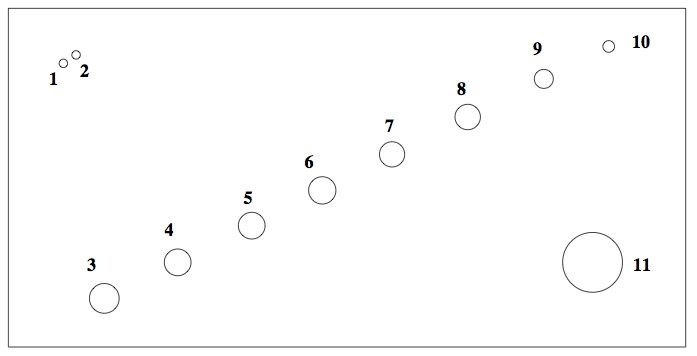
\includegraphics[width = 7cm]{img/klotz.jpeg}
		\caption{Aufbau der gest"orten Probe \label{fig:klotz}}
	\end{wrapfigure}

	Anschlie"send wird ein Acrylblock mit verschiedenen Bohrungen untersucht.
	Durch Nutzung des Impuls-Echo-Verfahrens wird dabei mit einem A-Scan der Abstand der Bohrungen zur Oberfl"ache des Glases bestimmt.
	Durch Messungen, ausgehend von Ober- und Unterseite kann dann der Durchmesser der Bohrungen bestimmt werden.
	Abbildung \ref{fig:klotz} zeigt schematisch den Aufbau der Probe.

	Zus"atzlich zum A-Scan wird hier ein B-Scan durchgef"uhrt.
	Bei langsamer Bewegung der Sonde "uber eine Seite der Probe kann so die Lage der Bohrungen visualisiert werden.
	Hier werden alle drei Sonden benutzt und die entsprechenden Bilder werden verglichen. \\

	Schlie"slich wird ein Modell des menschlichen Auges mit Hilfe der Ultraschallsonden vermessen.
	Durch den inneren Aufbau des Modells sind insgesamt vier Aplitudenpeaks zu erwarten, die durch Reflexion entstehen.
	Der erste Peak entspricht dabei einer Reflexion an der Iris, der zweite und dritte Peak einer Reflexion an der Vorder- bzw. R"uckseite der Linse, die durch die verschiedenen Schallgeschwindigkeiten in Glas und Augenfl"ussigkeit hervorgerufen wird.
	Der letzte Peak entspricht der Reflexion an der Retina.
	Durch die Laufzeitmessung und mit Kenntnis der Schallgeschwindigkeiten in Linse ($c_\mathrm{L} = \SI{2500}{\meter \per \second}$) und in der Fl"ussigkeit ($c_\mathrm{Fl} = \SI{1410}{\meter \per \second}$) k"onnen dann die Gr"o"sen im Auge bestimmt werden.